\section{DeepTune: Learning On Raw Program Code} \label{sec:DeepTune}

\begin{figure}
  \centering
  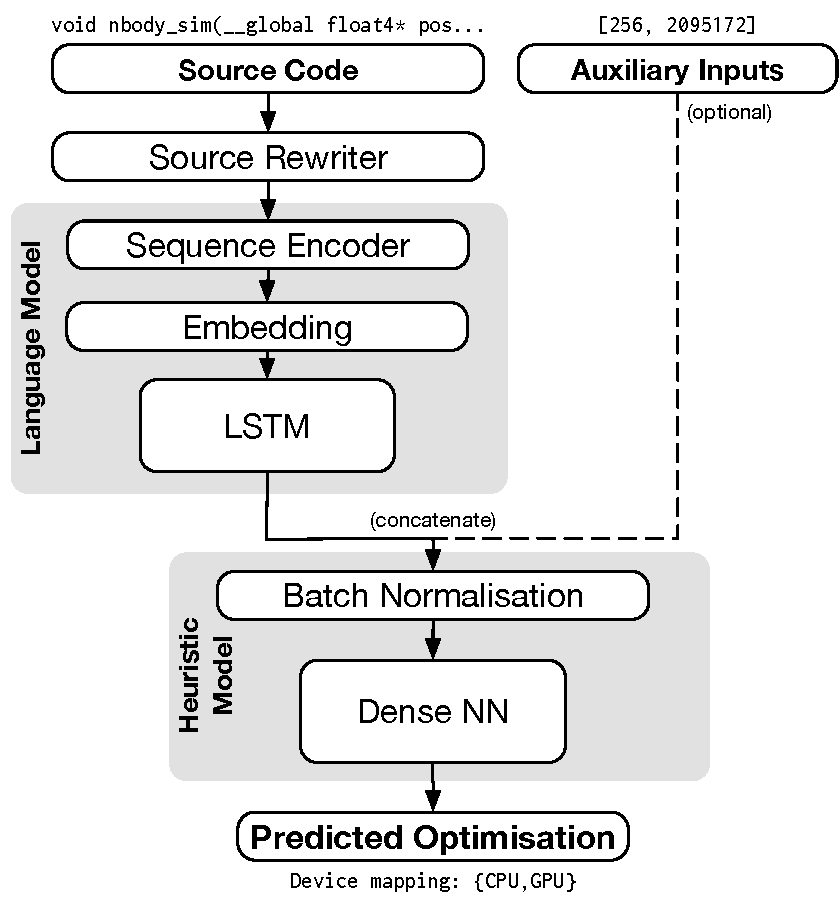
\includegraphics[width=\columnwidth]{img/deeptune} %
  \vspace{-2em}%
  \caption{%
    DeepTune architecture. Code properties are extracted from source code by the
    language model. They are fed, together with optional auxiliary inputs, to
    the heuristic model to produce the final prediction.%
  }%
  \label{fig:deeptune}
\end{figure}


DeepTune is an end-to-end machine learning pipeline for optimisation heuristics. Its primary input is the source code of a program to be optimised, and through a series of neural networks, it directly predicts the optimisation which should be applied. By learning on source code, our approach is not tied to a specific compiler, platform, or optimisation problem. The same design can be reused to build multiple heuristics. The most important innovation of DeepTune is that it forgoes the need for human experts to select and tune appropriate features.


\subsection{System Overview}

Figure~\ref{fig:deeptune} provides an overview of the system. A source re-writer removes semantically irrelevant information (such as comments) from the source code of the target program and passes it to a language model. The language model converts the arbitrary length stream of code into a fixed length vector of real values which fully capture the properties and structure of the source, replacing the role of hand designed features. We then optionally concatenate this vector with auxiliary inputs, which allow passing additional data about runtime or architectural parameters to the model for heuristics which need more than just compile-time information. Finally, a standard feed-forward network is used to predict the best heuristic parameters to optimise the program.

DeepTune is open source\footnote{DeepTune is available at: \url{https://chriscummins.cc/deeptune}}. We implemented the model in Keras, with TensorFlow~\cite{Abadi} and Theano~\cite{Bergstra2011} back-ends.


\subsection{Language Model}

Learning effective representations of source code is a difficult task. A successful model must be able to:
%
\begin{itemize}
  \item derive semantic and syntactic patterns of a programming language entirely from sample codes;
  \item identify the patterns and representation in source codes which are relevant to the task at hand; and
  \item discriminate performance characteristics arising from potentially subtle differences in similar codes.
\end{itemize}
%
To achieve this task, we employ state-of-the-art language modelling techniques, coupled with a series of generic, language agnostic code transformations.

\subsubsection{Source Re-writer} To begin with, we apply a series of \emph{source normalising} transformations extended from our previous work~\cite{Cummins2017a}. These transformations, implemented as an LLVM pass, parse the AST, removing conditional compilation, then rebuild the input source code using a consistent code style and identifier naming scheme. The role of source normalisation is to simplify the task of modelling source code by ensuring that trivial semantic differences in programs such as the choice of variable names or the insertion of comments do not affect the learned model. Figures~\ref{subfig:source_in} and~\ref{subfig:source_out} show the source rewriting applied to a simple program.

\subsubsection{Sequence Encoder}  We encode source code as a sequence of integers for interpretation by neural networks, where each integer is an index into a predetermined vocabulary. In~\cite{Cummins2017a}, a character based vocabulary is used. This minimises the size of the vocabulary, but leads to long sequences which are harder to extract structure from. In~\cite{Allamanis2013a}, a token based vocabulary is used. This leads to shorter sequences, but causes an explosion in the vocabulary size, as every identifier and literal must be represented uniquely.

We designed a hybrid, partially tokenised approach. This allows common multi-character sequences such as \texttt{float} and \texttt{if} to be represented as unique vocabulary items, while literals and other infrequently used words are encoded at the character level.

We first assembled a candidate vocabulary $V_c$ for the OpenCL programming language containing the 208 data types, keywords, and language builtins of the OpenCL programming language. We then derived the subset of the candidate vocabulary $V \in V_c$ which is required to encode a corpus of 45k lines of GPGPU benchmark suite kernels. Beginning with the first character in the corpus, our algorithm consumes the longest matching sequence from the candidate vocabulary. This process continues until every character in the corpus has been consumed. The resulting derived vocabulary consists of 128 symbols which we use to encode new program sources. Figure~\ref{subfig:source_vocab} shows the vocabulary derived for a single input source code Figure~\ref{subfig:source_out}.

\lstset{language=[OpenCL]C}
\begin{figure}
  \centering %
  \subfloat[%
    An example, short OpenCL kernel, taken from Nvidia's \emph{streamcluster}.%
  ]{%
    \noindent\mbox{\parbox{\columnwidth}{%
      \lstinputlisting[nolol,label=subfig:source_in]{lst/source_in}%
    }}%
  }\\%
  \subfloat[%
    The \emph{streamcluster} kernel after source rewriting. Variable and
    function names are normalised, comments removed, and code style enforced.%
  ]{%
    \noindent\mbox{\parbox{\columnwidth}{%
      \lstinputlisting[nolol,label=subfig:source_out]{lst/source_out}%
    }}%
  }\\%
  \subfloat[%
    Derived vocabulary, ordered by their appearance in the
    input~\protect\subref{subfig:source_out}. The vocabulary maps tokens to
    integer indices.%
  ]{%
    \footnotesize
\begin{tabular}{l l | l l | l l}
  \toprule
  \textbf{idx} & \textbf{token} & \textbf{idx} & \textbf{token} & \textbf{idx} & \textbf{token} \\
  \midrule
  \texttt{1} & \texttt{`\_\_kernel'} & \texttt{10} & \texttt{`,'} & \texttt{19} & \texttt{`const'} \\
  \texttt{2} & \texttt{` '} & \texttt{11} & \texttt{`short'} & \texttt{20} & \texttt{`d'} \\
  \texttt{3} & \texttt{`void'} & \texttt{12} & \texttt{`b'} & \texttt{21} & \texttt{`='} \\
  \texttt{4} & \texttt{`A'} & \texttt{13} & \texttt{`int'} & \texttt{22} & \texttt{`get\_global\_id'} \\
  \texttt{5} & \texttt{`('} & \texttt{14} & \texttt{`c'} & \texttt{23} & \texttt{`0'} \\
  \texttt{6} & \texttt{`\_\_global'} & \texttt{15} & \texttt{`)'} & \texttt{24} & \texttt{`;'} \\
  \texttt{7} & \texttt{`char'} & \texttt{16} & \texttt{`\{'} & \texttt{25} & \texttt{`['} \\
  \texttt{8} & \texttt{`*'} & \texttt{17} & \texttt{`\textbackslash n'} & \texttt{26} & \texttt{`]'} \\
  \texttt{9} & \texttt{`a'} & \texttt{18} & \texttt{`\space\space'} & \texttt{27} & \texttt{`\}'} \\
  \bottomrule
\end{tabular}%
%
    \label{subfig:source_vocab}%
  }\\%
  \subfloat[%
    Indices encoded kernel sequence. Sequences may be padded to a fixed length
    by repeating an out-of-vocabulary integer (e.g. -1).%
  ]{%
    \rowcolors{2}{white}{gray!25}
\begin{tabular}{l l l l l l l l l l l}
	\toprule
	\texttt{01} & \texttt{02} & \texttt{03} & \texttt{02} & \texttt{04} & \texttt{05} & \texttt{06} & \texttt{02} & \texttt{07} & \texttt{08} & \texttt{02} \\
	\texttt{09} & \texttt{10} & \texttt{02} & \texttt{11} & \texttt{02} & \texttt{12} & \texttt{10} & \texttt{02} & \texttt{13} & \texttt{02} & \texttt{14} \\
	\texttt{15} & \texttt{02} & \texttt{16} & \texttt{17} & \texttt{18} & \texttt{19} & \texttt{02} & \texttt{13} & \texttt{02} & \texttt{20} & \texttt{02} \\
	\texttt{21} & \texttt{02} & \texttt{22} & \texttt{05} & \texttt{23} & \texttt{15} & \texttt{24} & \texttt{17} & \texttt{18} & \texttt{09} & \texttt{25} \\
	\texttt{20} & \texttt{26} & \texttt{02} & \texttt{21} & \texttt{02} & \texttt{12} & \texttt{24} & \texttt{17} & \texttt{27} & \multicolumn{2}{l}{\texttt{<pad\ldots>}} \\
	\bottomrule
\end{tabular}
%
    \label{subfig:source_enc}%
  }%
  \caption[Deriving a vocabulary encoding from an OpenCL source code]{%
    Deriving a tokenised $1$-of-$k$ vocabulary encoding from an OpenCL source
    code.%
  }%
  \label{fig:encoding}%
\end{figure}


\subsubsection{Embedding} During encoding, tokens in the vocabulary are mapped to unique integer values, e.g. \texttt{float} $\rightarrow 0$, \texttt{int} $\rightarrow$ 1. The integer values chosen are arbitrary, and offer a \emph{sparse} data representation, meaning that a language model cannot infer the relationships between tokens based on their mappings. This is in contrast to the \emph{dense} representations of other domains, such as pixels in images, which can be interpolated between to derive the differences in colours.

To mitigate this, we use an \emph{embedding}, which translates tokens in a sparse, integer encoded vocabulary into a lower dimensional vector space, allowing semantically related tokens like \texttt{float} and \texttt{int} to be mapped to nearby points~\cite{Mikolov2013a,Baroni2014}. An embedding layer maps each token in the integer encoded vocabulary to a vector of real values. Given a vocabulary size $V$ and embedding dimensionality $D$, an embedding matrix $\bm{W_{E}} \in \mathbb{R}^{V \times D}$ is learned during training, so that an integer encoded sequences of tokens $\bm{t} \in \mathbb{N}^{L}$ is mapped to the matrix $\bm{T} \in \mathbb{R}^{L \times D}$. We use an embedding dimensionality $D = 64$.

\subsubsection{Sequence Characterisation} Once source codes have been encoded into sequences of embedding vectors, neural networks are used to extract a fixed size vector which characterises the entire sequence. This is comparable to the hand engineered feature extractors used in prior works, but is a \emph{learned} process that occurs entirely --- and automatically --- within the hidden layers of the network.

We use the the Long Short-Term Memory (LSTM) architecture~\cite{Hochreiter1997} for sequence characterisation. LSTMs implements a Recurrent Neural Network in which the activations of neurons are learned with respect not just to their current inputs, but to previous inputs in a sequence. Unlike regular recurrent networks in which the strength of learning decreases over time (a symptom of the \emph{vanishing gradients} problem~\cite{Pacanu2013}), LSTMs employ a \emph{forget gate} with a linear activation function, allowing them to retain activations for arbitrary durations. This makes them effective at learning complex relationships over long sequences~\cite{Lipton2015}, an especially important capability for modelling program code, as dependencies in sequences frequently occur over long ranges (for example, a variable may be declared as an argument to a function and used throughout).

We use a two layer LSTM network. The network receives a sequence of embedding vectors, and returns a single output vector, characterising the entire sequence.


\subsection{Auxiliary Inputs}

We support an arbitrary number of additional real valued \emph{auxiliary inputs} which can be optionally used to augment the source code input. We provide these inputs as a means of increasing the flexibility of our system, for example, to support applications in which the optimisation heuristic depends on dynamic values which cannot be statically determined from the program code~\cite{Ding2015,Stephenson2005}. When present, the values of auxiliary inputs are concatenated with the output of the language model, and fed into a heuristic model.


\subsection{Heuristic Model}

The heuristic model takes the learned representations of the source code and auxiliary inputs (if present), and uses these values to make the final optimisation prediction.

We first normalise the values. Normalisation is necessary because the auxiliary inputs can have any values, whereas the language model activations are in the range [0,1]. If we did not normalise, then scaling the auxiliary inputs could affect the training of the heuristic model. Normalisation occurs in batches. We use the normalisation method of%~\cite{Ioffe2015a}
, in which each scalar of the heuristic model's inputs $x_1 \ldots x_n$ is normalised to a mean 0 and standard deviation of 1:
%
\begin{equation}
x_i' = \upgamma_i \frac{x_i - E(x_i)}{\sqrt{Var(x_i)}} + \beta_i
\end{equation}
%
where $\upgamma$ and $\beta$ are scale and shift parameters, learned during training.

The final component of DeepTune is comprised of two fully connected neural network layers. The first layer consists of 32 neurons. The second layer consists of a single neuron for each possible heuristic decision. Each neuron applies an activation function $f(x)$ over its inputs. We use rectifier activation functions $f(x) = \max(0, x)$ for the first layer due to their improved performance during training of deep networks~\cite{Nair2010}. For the output layer, we use sigmoid activation functions $f(x) = \frac{1}{1+e^{-x}}$ which provide activations in the range $[0,1]$.

The activation of each neuron in the output layer represents the model's confidence that the corresponding decision is the correct one. We take the $\argmax$ of the output layer to find the decision with the largest activation. For example, for a binary optimisation heuristic the final layer will consist of two neurons, and the predicted optimisation is the neuron with the largest activation.


\subsection{Training the network}

DeepTune is trained in the same manner as prior works, the key difference being that instead of having to manually create and extract features from programs, we simply use the raw program codes themselves.

The model is trained with Stochastic Gradient Descent (SGD), using the Adam optimiser~\cite{Kingma2015}. For training data $X_1 \ldots X_n$, SGD attempts to find the model parameters $\Theta$ that minimise the output of a loss function:
%
\begin{equation}
\Theta = \argmin_{\Theta} \frac{1}{n} \sum_{i=1}^{n} \ell \left(X_i, \Theta \right)
\end{equation}
%
where loss function $\ell \left(x, \Theta \right)$ computes the logarithmic difference between the predicted and expected values.

To reduce training time, multiple inputs are \emph{batched} together and are fed into the neural network simultaneously, reducing the frequency of costly weight updates during back-propagation. This requires that the inputs to the language model be the same length. We pad all sequences up to a fixed length of 1024 tokens using a special padding token, allowing matrices of \texttt{batch\_size} $\times$ \texttt{max\_seq\_len} tokens to be processed simultaneously. We note that batching and padding sequences to a maximum length is only to improve training time. In production use, sequences do not need to be padded, allowing classification of arbitrary length codes.
es.
